\section{Meanshift和Camshift}

\subsection{Meanshift背后的数学思想}
Meanshift在统计学中是一种聚类(clustering)方法

Meanshift在目标跟踪上的的核心思想是,让目标和采样区域的颜色、纹理等特征尽量符合。

在机器学习领域,我们通常设计一个目标函数,通常也叫做``损失函数(Loss functions)'',以最小化目标函数的值作为优化目标。

\subsection{为目标跟踪设计的损失函数}

优化目标:需要跟踪的物体的特征和周围的新的某一区域特征相符合
\begin{center}
    $\downarrow$
\end{center}

物体HSV分布PDF和区域HSV PDF分布相符合。

\vspace{2em}

如何求PDF $\Rightarrow$ ?  KDE(Kernel Density Estimation)

巴氏系数

\begin{equation}
    \rho = \int \sqrt{p \cdot q} \d z
\end{equation}

\subsection{如何由样本估计概率分布?-- 非参数估计之核密度估计}

设 $(x_1, x_2, \dots, x_n)$ 是独立同分布的样本,则核密度估计给出

\begin{equation}
    \hat{f_h} (x) = \frac{1}{n} \sum K_h(x - x_i)
\end{equation}
\begin{figure}
    \centering
    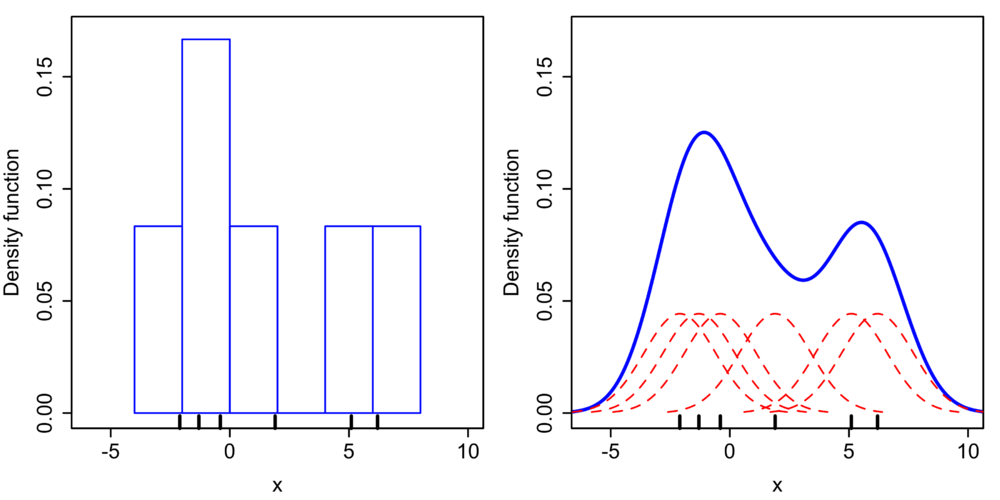
\includegraphics[width=0.618\textwidth]{images/Comparison_of_1D_histogram_and_KDE.png}
    \caption{左:直方图,右:核密度估计}
\end{figure}
